\begin{proof}
    Suppose that the statement is false. This conditional statement being false means that \(B\) and \(C\) are two points such that:
    \begin{itemize}
        \item for every pair \(D,E\) of intersection points of a generic line through \(O\) with the two sides of the angle, \(\TriangleArea{ABC} \leq \TriangleArea{ADE}\) (that is, the triangle \(\Triangle{ABC}\) has minimal area);
        \item \(\Segment{BO} \ne \Segment{CO}\).
    \end{itemize}
    Pass a line through \(O\) such that \(\Segment{DO} = \Segment{EO}\) (where \(D\) and \(E\) are the intersection points of the line with the two sides of the angle). Clearly, \(B \neq D\) and \(C \neq E\) (otherwise it would be true that \(\Segment{BO} = \Segment{CO}\)).
    \begin{figure}[H]
        \centering
        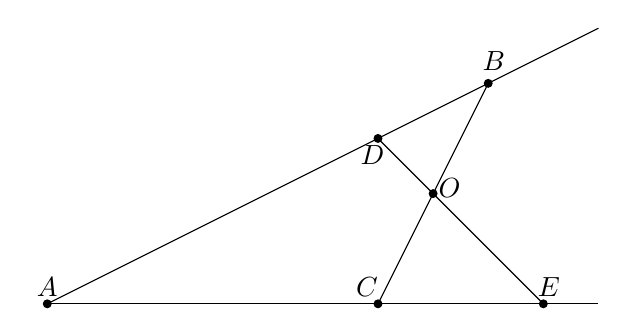
\begin{tikzpicture}[scale=0.7]
    \draw (0,0) -- (10,0);
    \draw (0,0) -- (10,5);
    \draw (8,4) -- (6,0);
    \draw (6,3) -- (9,0);
    \filldraw (0,0) circle[radius=2pt];
    \draw (0,0.3) node {$A$};
    \filldraw (7,2) circle[radius=2pt];
    \draw (7.3,2.1) node {$O$};
    \filldraw (8,4) circle[radius=2pt];
    \draw (8.1,4.4) node {$B$};
    \filldraw (6,0) circle[radius=2pt];
    \draw (5.8,0.3) node {$C$};
    \filldraw (6,3) circle[radius=2pt];
    \draw (5.9,2.7) node {$D$};
    \filldraw (9,0) circle[radius=2pt];
    \draw (9.1,0.3) node {$E$};
\end{tikzpicture}
    \end{figure}
    Draw a line through \(D\) and parallel to \(\Segment{AC}\). Let \(B'\) be the intersection between this line and the extension of \(\Segment{BC}\). Clearly, it's true that \(\TriangleArea{CEO} = \TriangleArea{B'DO}\) (since \(\Triangle{CEO} \cong \Triangle{B'DO}\)).
    \begin{figure}[H]
        \centering
        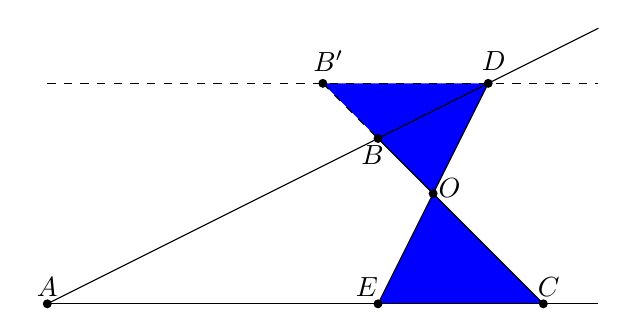
\begin{tikzpicture}[scale=0.7]
    \fill[color=blue] (5,4) -- (7,2) -- (8,4) -- cycle;
    \fill[color=blue] (7,2) -- (6,0) -- (9,0) -- cycle;
    \draw (0,0) -- (10,0);
    \draw (0,0) -- (10,5);
    \draw (8,4) -- (6,0);
    \draw (6,3) -- (9,0);
    \draw [dashed] (0,4) -- (10,4);
    \draw [dashed] (5,4)-- (6,3);
    \filldraw (0,0) circle[radius=2pt];
    \draw (0,0.3) node {$A$};
    \filldraw (7,2) circle[radius=2pt];
    \draw (7.3,2.1) node {$O$};
    \filldraw (8,4) circle[radius=2pt];
    \draw (8.1,4.4) node {$D$};
    \filldraw (6,0) circle[radius=2pt];
    \draw (5.8,0.3) node {$E$};
    \filldraw (6,3) circle[radius=2pt];
    \draw (5.9,2.7) node {$B$};
    \filldraw (9,0) circle[radius=2pt];
    \draw (9.1,0.3) node {$C$};
    \filldraw (5,4) circle[radius=2pt];
    \draw (5.1,4.4) node {$B'$};
\end{tikzpicture}
    \end{figure}
    Moreover, \(\TriangleArea{BB'D} \neq 0\), since \(B \neq D\). Therefor, \(\TriangleArea{BDO} < \TriangleArea{CEO}\).\par
    I also know that \(\TriangleArea{ADE} = \TriangleArea{ABC} - \TriangleArea{CEO} + \TriangleArea{BDO}\).
    \begin{figure}[H]
        \centering
        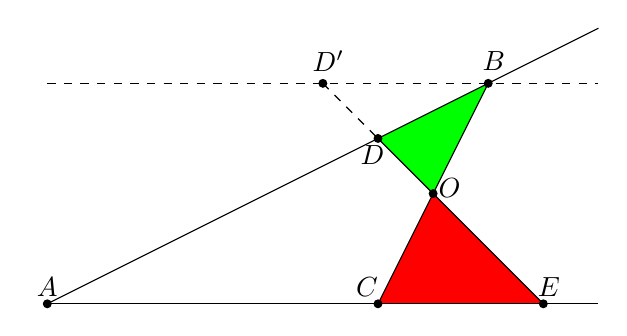
\begin{tikzpicture}[scale=0.7]
    \fill[color=green] (6,3) -- (7,2) -- (8,4) -- cycle;
    \fill[color=red] (7,2) -- (6,0) -- (9,0) -- cycle;
    \draw (0,0) -- (10,0);
    \draw (0,0) -- (10,5);
    \draw (8,4) -- (6,0);
    \draw (6,3) -- (9,0);
    \draw [dashed] (0,4) -- (10,4);
    \draw [dashed] (5,4)-- (6,3);
    \filldraw (0,0) circle[radius=2pt];
    \draw (0,0.3) node {$A$};
    \filldraw (7,2) circle[radius=2pt];
    \draw (7.3,2.1) node {$O$};
    \filldraw (8,4) circle[radius=2pt];
    \draw (8.1,4.4) node {$B$};
    \filldraw (6,0) circle[radius=2pt];
    \draw (5.8,0.3) node {$C$};
    \filldraw (6,3) circle[radius=2pt];
    \draw (5.9,2.7) node {$D$};
    \filldraw (9,0) circle[radius=2pt];
    \draw (9.1,0.3) node {$E$};
    \filldraw (5,4) circle[radius=2pt];
    \draw (5.1,4.4) node {$D'$};
\end{tikzpicture}
    \end{figure}
    Thus, \(\TriangleArea{ADE} < \TriangleArea{ABC}\) and I can conclude that \(\Triangle{ABC}\) has not a minimal area. Since I have a contradiction, I was wrong to assume that the statement was false: it must be true.
\end{proof}